\documentclass[conference]{IEEEtran}
\usepackage{interval}
\usepackage[inline]{enumitem}
\usepackage{stmaryrd}
\usepackage{amsmath}
\usepackage{graphicx}
\newcommand{\inhib}{\relbar\mapsfromchar}

\begin{document}
\subsection{Arbiter implementation}

In order to use the priority scores determined by our scheme to allocate the data transfer budget to the highest scoring logical qubits, we need a way to identify the $k$ logical qubits with the highest priority scores out of the $n$ that are competing to be decoded.
An arbiter circuit that implements the top-$k$ argmax of the $n$ priority scores based on arithmetic comparison of binary priority scores and multiplexing of qubit indexes would incur a significant area cost for the budget current integration density of superconducting cells allows, especially as the number of logical qubits $n$ and number of supported priority levels increases.
Fortunately, designs like this one that consist of comparisons can be implemented efficiently using temporal computing, a logic scheme where information is represented as the time of arrival of signals, allowing priority scores of any number of bits to be supported by a single wire. 
Specifically, we design our arbiter using the paradigm of race logic \cite{racelogic}, for which a mapping of it's primitives to superconducting cells was provided in \cite{sfq_race}.

For the comparator module we base the arbiter on, we make use of three race logic primitives.
The first two primitives are First Arrival (FA) and Last Arrival (LA), which perform the equivalent of $\min$ and $\max$ operations of the temporally encoded values.
FA will fire upon the first pulse it receives in one of it's input ports and reset upon receiving a second pulse on it's other input port, whereas LA both fires and resets upon receiving the second pulse.
In SFQ they are implemented with an inverted Muller C cell and a regular C cell respectively.
We have tuned these cells to have very similar delays, so differences in their propagation speed do not lead to the need for synchronizing signals inside the arbiter.
The third primitive is Inhibit (INH), that has two input ports $a$ and $b$ and propagates a pulse received on $b$ only if it arrives before a pulse on $a$ does.
Typically Inhibit is implemented using a clocked inverter cell, however because we need only a boolean signal of whether $b$ arrived before $a$ and not a temporal signal of when $b$ arrived for our purposes, we substitute it for the cheaper DRO cell, and assign $a$ to the DRO's clock port and $b$ to it's data input port.
In the case $a$ and $b$ arrive very close to each other, they will both represent the same priority score and their comparison will be a tie, in which case either the DRO firing or not are both valid for our purposes.
With these primitives we can design the comparator module of size 2 that will be the building block of our arbiter.

The comparator module's ports consist of four pairs, each pair consisting of a data port and a select port.
It provides the functionality for both a forward pass that uses the data ports to sort the input priority scores and a backward pass that uses the select ports to route signals to go down the same path data signals did in the forward pass.
The forward pass connects the $x_0$ and $x_1$ input wires which encode priority scores to FA, LA and INH cells.
The outputs of FA and LA connect to the $x_{min}$ and $x_{min}$ output ports of the comparator, propagating the earliest and latest pulses from the inputs respectively.
The output of the INH cell goes to the data input of two DROC cells, to prepare them for the backward pass.
In the backward pass input ports $sel_{min}$ and $sel_{max}$ are connected to the clock ports of the DROC cells.
The outputs of the DROC pair are merged such that a pulse from $sel_{min}$ is routed to $sel_0$ if the DROC pair stores a pulse from the INH, meaning that signal $x_0$ arrived before $x_1$, and to $sel_1$ otherwise.
Similarly, a signal from $sel_{max}$ goes to $sel_1$ if $x_0$ arrived before $x_1$ and to $sel_0$ otherwise.

Fig\ref{fig:comp} shows an example of the comparator module's operation with the routes the 
various signals took.
Fig~\ref{fig:comcirc} shows the gate level implementation of the comparator module.
As it can be seen, only a handful of gates are needed compared to what a bit parallel arithmetic implementation would require.

To build the full arbiter that provides the functionality of top-$k$ argmax, we arrange comparator modules in the configuration of a bitonic sorter.
Fig~\ref{fig:sort4} shows the arrangement for a 4 element bitonic sorter.
Also shown is the path of the latest arriving encoded priority score through the sorter and the path a select signal given at the highest position of the sorter's final layer takes through the comparator modules to fire at the select port of the first layer, denoting the argmax of the data input pulses.

Scaling the bitonic sorter configuration to the number $n$ of priority scores we need to evaluate would work for a top-$k$ argmax if we first send the temporally encoded priority scores for all $n$ qubits as input pulses for the forward pass and after that fire pulses at the select ports of the final layer corresponding to the $k$ largest positions.
These would get routed to the select ports of the first layer corresponding to the $k$ largest scores entered in the data ports, providing a binary flag representation of the argmax that can be used without additional decoding.
However, a large part of this structure would be wasted on comparators sorting signals that cannot be in the top-$k$, and thus are not needed.
After removing the unnecessary comparators we are left with a structure where the data signals are split in groups of length $k$ and each group goes through a full bitonic sorter of size $k$.
The number of data signals is then cut in half by selecting the $k$ largest outputs from each pair of $k$-sized sorters.
For every comparator that performs this reduction only the $max$ pair of data/select ports is connected to the next layer, whereas the $x_{min}$ and $sel_{min}$ are left unconnected.
The $\frac{n}{2}$ signals left go through a similar sort and reduce process, although subsequent blocks of size $k$ sorters require less comparators. 
After the final reduction $k$ signals will be left, from which the select signals for the top-$k$ will originate.
Fig~\ref{fig:arb16} shows such a sparse arbiter that selects the top 4 out of 16 signals.

\subsection{Reset scheme}

After an execution of the arbiter, some of the DRO and DROC cells could be still storing a pulse, which needs to be cleared before the next execution can occur.
The FA and LA cells have all received a pulse in both of their input ports during execution, thus they are already reset.
As the arbiter only operates once per decode cycle, hundreds of nanoseconds pass between executions, providing ample time to reset the DRO and DROC cells.
Although an external reset signal could be used, it would require more complicated and expensive cells that have an additional reset port and incur splitting overhead to connect the reset signal to every cell.
To avoid this, we design a data-driven reset scheme.
This enables us to return all cells to their original state by only inserting signals to already existing ports in the design, with no changes to it's internals.
The first step of the reset scheme resets all the inhibit DRO cells via a forward pass of the arbiter.
When a comparator module gets a pulse at $x_0$ first and at $x_1$ after, it's inhibit DRO will fire after receiving a pulse at the data port and thus clear.
Additionally in this case the comparator will propagate the data inputs with the same order it received them.

We make use of these properties by inserting a linearly increasing sequence of pulses in the data input ports of the arbiter, meaning that input $i+1$ will receive a pulse a fixed time after input $i$.
Due to the arrangement of comparators in a bitonic sorter, the order of pulses will remain the same through every comparator layer, as it is already sorted, and also every comparator will receive a pulse at input $x_0$ before $x_1$, clearing it's DRO.
Since every inhibit DRO in the design fired, all DROC cells in the arbiter's comparators will store a pulse, setting the stage for the second step of the reset scheme.
In this step, we insert a pulse at the select signals for the top $k$ scores in the final layer, as well as the unused $sel_{min}$ ports of the comparators in every reduction layer.
Together these $n$ select signals will pass through every select port in their path towards the first layer, causing every DROC to fire and clear in the process.
The linearly increasing sequence of pulses for the first step can be easily produced using a splitter chain, where a pulse entering the $i$-th chain link will be split into two pulses, one being merged into the $i$-th input of the arbiter and going through a few JTL to add a bit of delay before entering the $i+1$ part of the splitter chain.
To support the second step only a splitter tree of size $n$ for the reset signal is needed.

\subsection{Priority score evaluation}

To evaluate the priority score of a logical qubit from it's syndromes, the first step is producing the complex flags for each ancilla qubit.
We use the same basic gate configuration as \cite{btwc} for this end, and since the circuit is not pipelined but instead gets run once all the way through every decode cycle, we route in a clock-follows-data fashion (concurrent clocking), which lets us avoid inserting buffer gates to deal with logic depth imbalance.
The complex flags from each ancilla qubit of the same type are agregated into a single flag for each quadrant that tracks whether any qubit belonging to the quadrant is the center of the complex clique.
This agregation is done very efficiently by connecting the complex flag wires of each quadrant's ancillas as inputs to a merger tree of the same size.
Fig~\ref{fig:mtree} shows the connections of complex flags to the merger trees for an example surface code.
Since merger cells are both clock-less and stateless, this is the cleanest way to combine a set of signals.
Because more than one pulse might reach the output of the merger tree if multiple input complex flags fire, a DRO is placed at the output of each tree.
This way any number of pulses at the output simply set the state of the DRO to one, making it fire a single pulse when the clock triggers it.

This produces complex flags $C_i, i \in \interval{0}{3}$ for each of the four quadrants, which in combination with the flag $T$ for whether the qubit is before a T gate will be encoded into a priority score using the system described above.
The priority score mapping used for this example is shown in Table~\ref{tab:scores}.
To start, the four binary complex flags are sorted so all the 1s are at the beginning, resulting in signals $S_i, i \in \interval{0}{3}$ for which $S_{i} \ge S_{i+1}$.
This sort uses a size 4 bitonic sorter similar to the one shown for the arbiter, but since the select part is not needed it becomes much cheaper, needing only 12 FA or LA cells and 12 splitters for the whole sorter.
Since this small sorter is only active for a few picoseconds in a period of hundreds of nanoseconds, a small internal leakage can be used to reset the FA and LA cells after operation.
In order to encode the priority score into a temporal signal for the arbiter, we pass the $S$ flags and a dual rail representation of the $T$ flag into a controllable delay module.

The basic block of the delay module is shown in Figure~\ref{fig:delblock}.
A control signal determines which of two paths with different delays a pulse arriving at the clock port of the DROC will take before being merged to the output of the block.
The additional delay incured when the control signal is set is configured by the number of JTL cells added to the longer path.
Using the $S$ flags as the control inputs, the temporal encoder consists of two chains of delay blocks.
We set the JTL delay of block $B_{i,t}, i \in \interval{0}{3}, t \in \interval{0}{1}$ such that the sum of the JTL delays for it and the blocks before it sum up to the temporal encoding for number of active quadrants equal to $i+1$ and $T = t$.
The circuit diagram for the temporal encoder and the additional delay of each block to encode the mapping of Table~\ref{tab:scores} is shown in Figure~\ref{fig:tempenc}.
The two chains produce two temporal encodings, one corresponding to $T$ being active and one for $T$ inactive.
The outputs of the chains connect to the clock port of a DRO each, the first DRO having it's data port connected to the positive wire of the dual rail $T$ flag and the other to it's negative wire.
Thus the temporal encoding is multiplexed by the $T$ flag to enter the arbiter.

\begin{figure}[h!]
  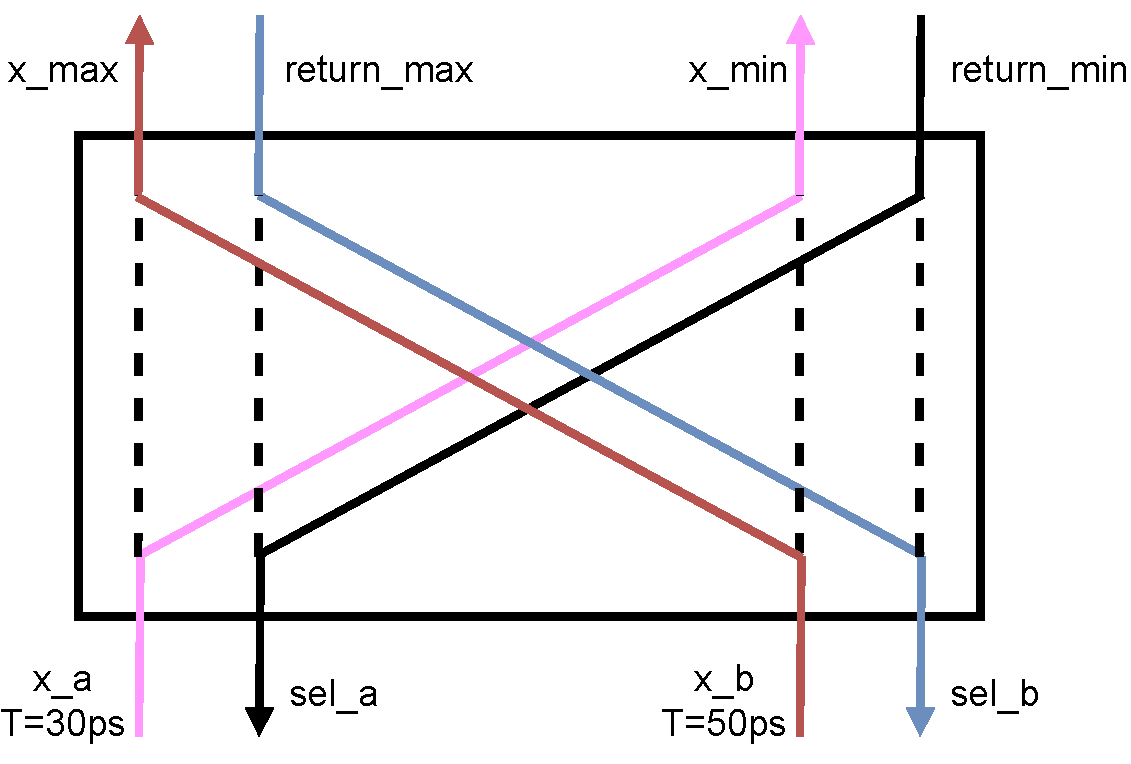
\includegraphics[width=0.5\textwidth]{figures/comparator.drawio.pdf}
  \caption{}
  \label{fig:comp}
\end{figure}

\begin{figure}[h!]
  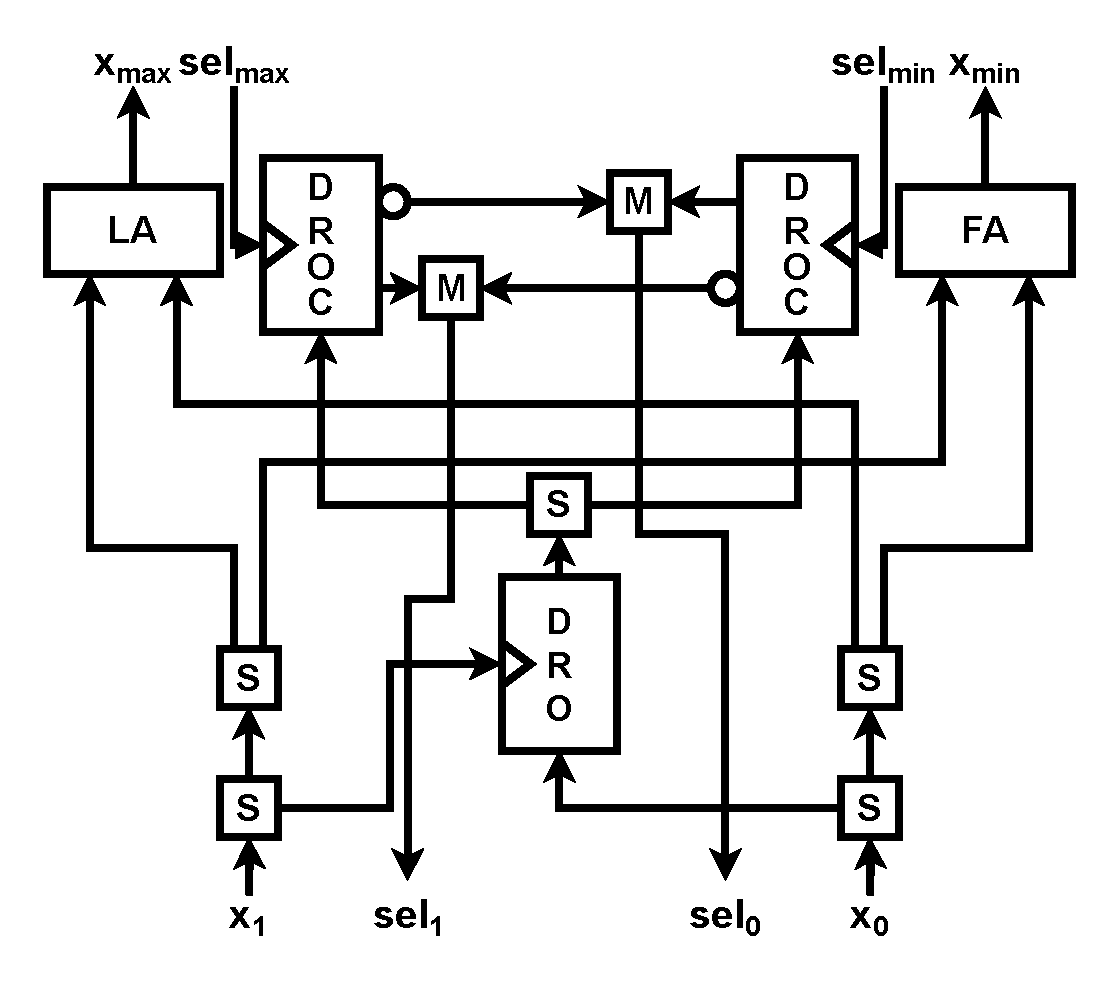
\includegraphics[width=0.5\textwidth]{figures/circuit_comparator.drawio.pdf}
  \caption{}
  \label{fig:comcirc}
\end{figure}

\begin{figure}[h!]
  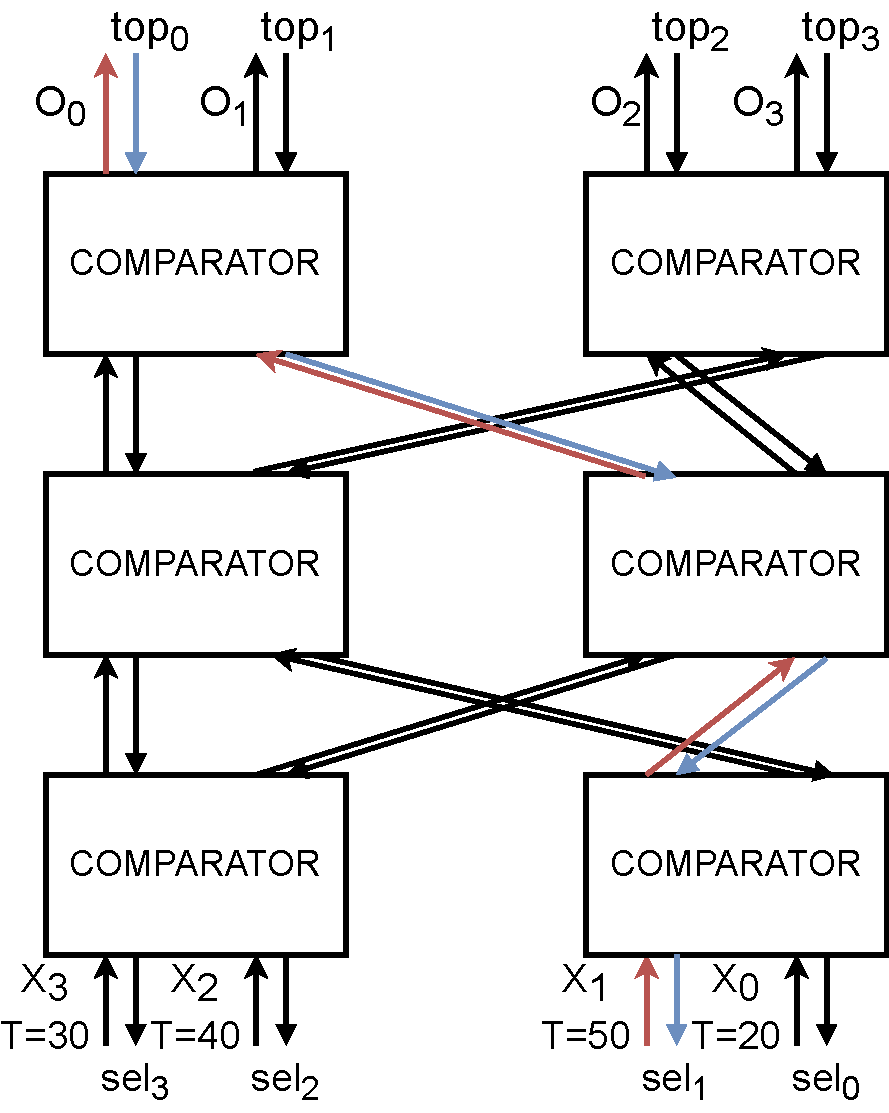
\includegraphics[width=0.5\textwidth]{figures/sort4.drawio.pdf}
  \caption{}
  \label{fig:sort4}
\end{figure}

\begin{figure}[h!]
  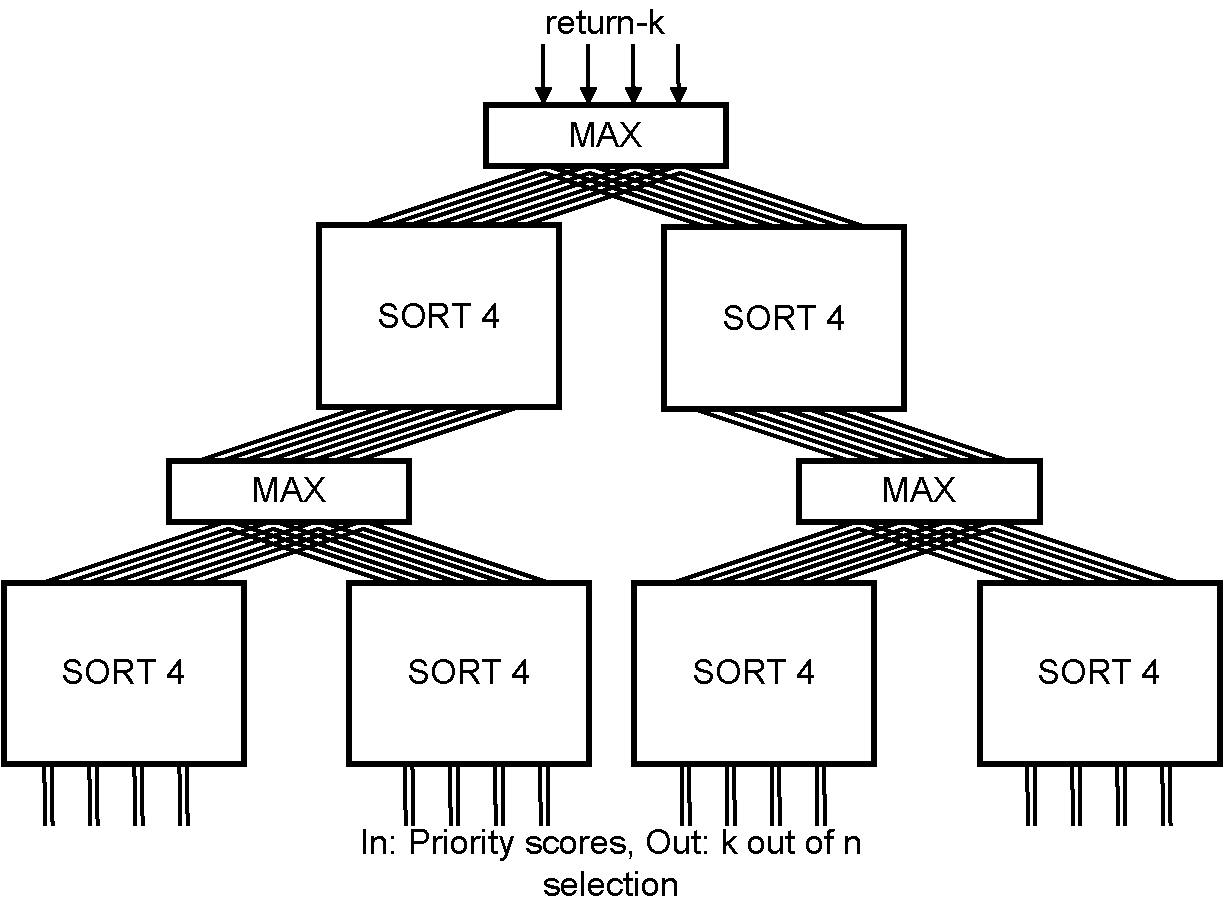
\includegraphics[width=0.5\textwidth]{figures/arbiterk4n16.drawio.pdf}
  \caption{}
  \label{fig:arb16}
\end{figure}

\begin{figure}[h!]
  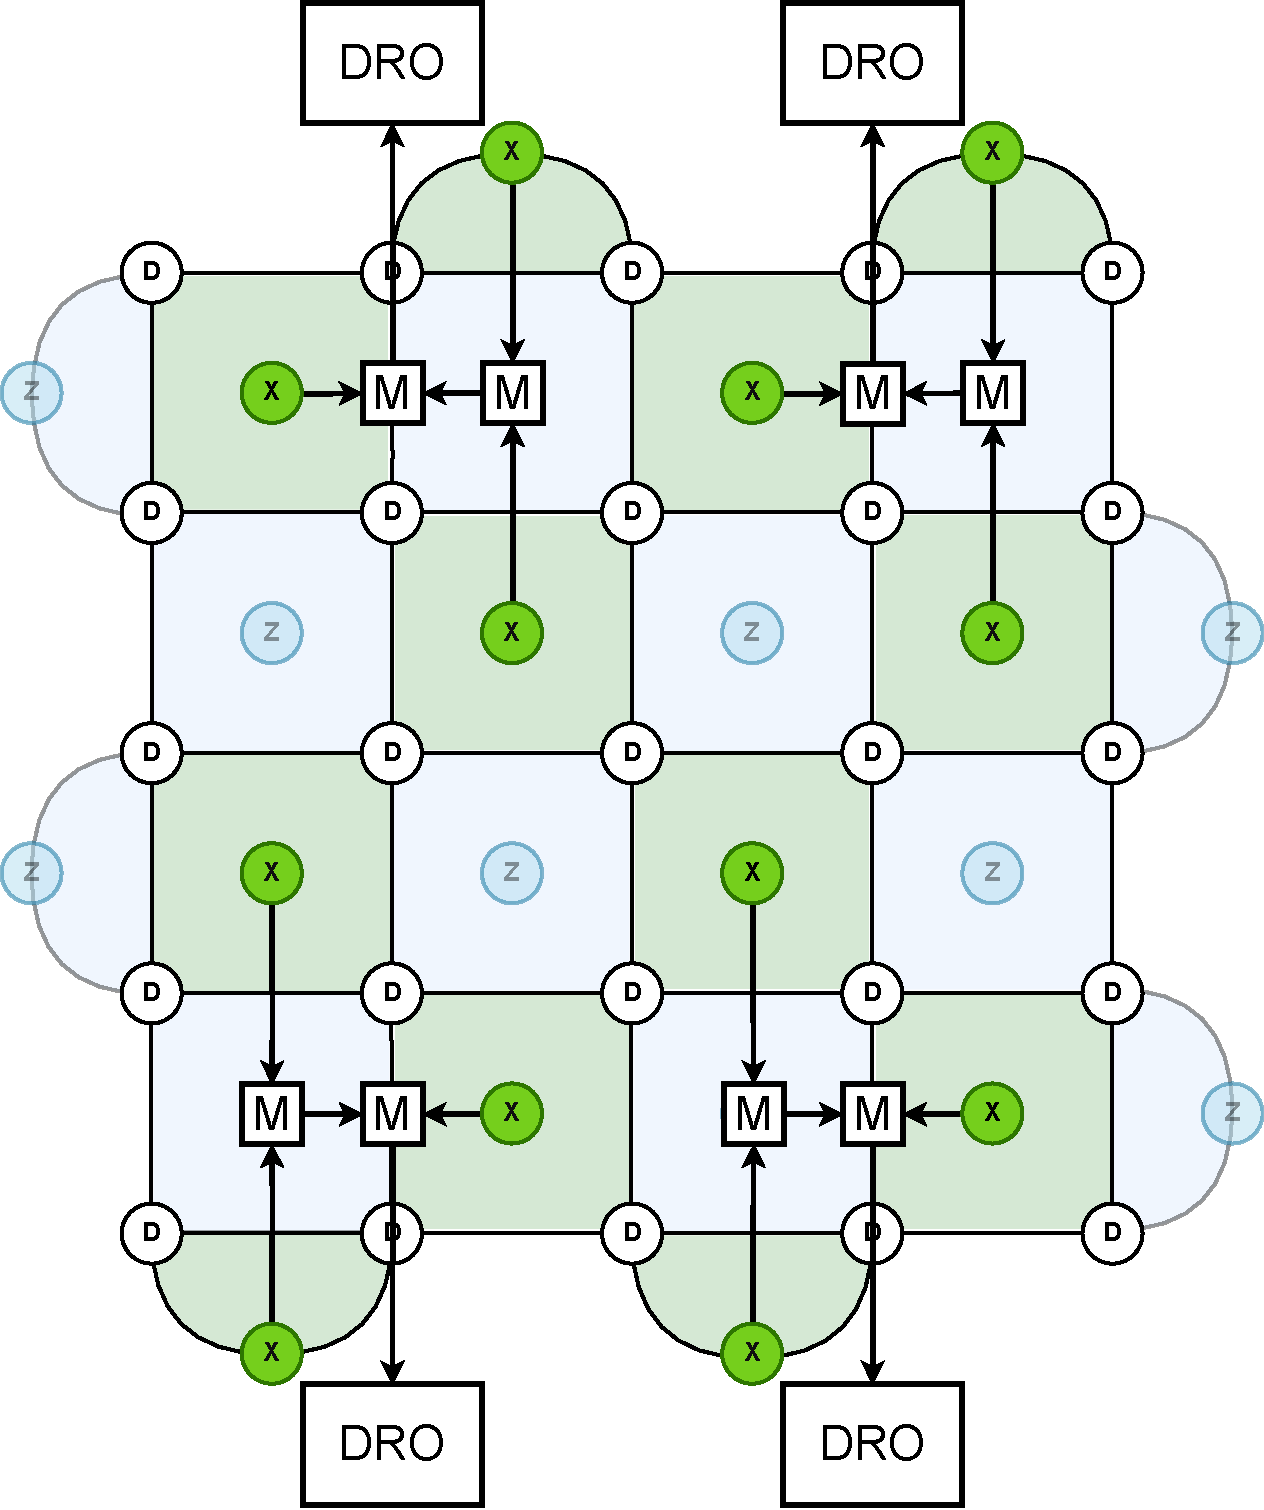
\includegraphics[width=0.5\textwidth]{figures/mtree.drawio.pdf}
  \caption{}
  \label{fig:mtree}
\end{figure}

\begin{figure}[h!]
  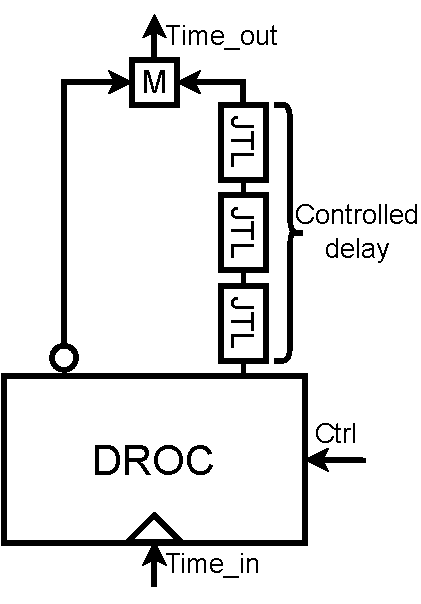
\includegraphics[width=0.5\textwidth]{figures/delay_block.drawio.pdf}
  \caption{}
  \label{fig:delblock}
\end{figure}

\begin{figure}[h!]
  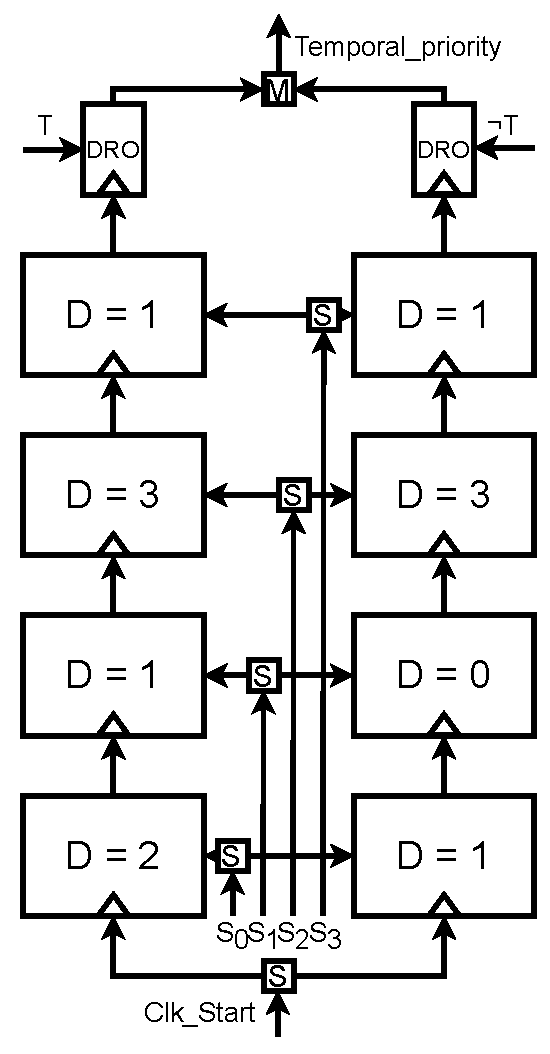
\includegraphics[width=0.5\textwidth]{figures/temporal_encoder.drawio.pdf}
  \caption{}
  \label{fig:tempenc}
\end{figure}

\end{document}

% @article{madhavan2014race,
%   title={Race logic: A hardware acceleration for dynamic programming algorithms},
%   author={Madhavan, Advait and Sherwood, Timothy and Strukov, Dmitri},
%   journal={ACM SIGARCH Computer Architecture News},
%   volume={42},
%   number={3},
%   pages={517--528},
%   year={2014},
%   publisher={ACM New York, NY, USA}
% }

% @ARTICLE{9380389,
%   author={Tzimpragos, Georgios and Volk, Jennifer and Vasudevan, Dilip and Tsiskaridze, Nestan and Michelogiannakis, George and Madhavan, Advait and Shalf, John and Sherwood, Timothy},
%   journal={IEEE Micro}, 
%   title={Temporal Computing With Superconductors}, 
%   year={2021},
%   volume={41},
%   number={3},
%   pages={71-79},
%   keywords={Superconducting logic circuits;Logic gates;Delays;Superconductivity;Semantics;Hardware;Josephson junctions},
%   doi={10.1109/MM.2021.3066377}}

